
%(BEGIN_QUESTION)
% Copyright 2012, Tony R. Kuphaldt, released under the Creative Commons Attribution License (v 1.0)
% This means you may do almost anything with this work of mine, so long as you give me proper credit

A pair of motor-driven compressors work in tandem to compress gas at an industrial ammonia production facility.  The control strategy is designed to evenly match the load between the two compressors, so that one is never working harder than the other, yet at the same time the two machines work together to maintain a common goal:

$$\includegraphics[width=15.5cm]{i01145x01.eps}$$

Identify the proper actions for each controller in this system, assuming direct-acting transmitters and motor controls that spin the motor at a faster speed with a greater 4-20 mA signal:

\vskip 10pt

FIC-236 = {\it direct} or {\it reverse}? \hskip 30pt SC-238 = {\it direct} or {\it reverse}? \hskip 30pt PIC-211 = {\it direct} or {\it reverse}?

\vskip 10pt

Suppose an operator calls you to examine this system and determine why the discharge pressure is not holding at setpoint.  According to the operator, everything was working fine yesterday, and had been working fine for months.  You go to the control room to view the display on the DCS, and you find these values:

% No blank lines allowed between lines of an \halign structure!
% I use comments (%) instead, so that TeX doesn't choke.

$$\vbox{\offinterlineskip
\halign{\strut
\vrule \quad\hfil # \ \hfil & 
\vrule \quad\hfil # \ \hfil & 
\vrule \quad\hfil # \ \hfil \vrule \cr
\noalign{\hrule}
%
% First row
{\bf Parameter} & {\bf FIC-236} & {\bf PIC-211}  \cr
%
\noalign{\hrule}
%
% Another row
PV & 29\% & 41\%  \cr
%
\noalign{\hrule}
%
% Another row
SP & 29\% & 60\%  \cr
%
\noalign{\hrule}
%
% Another row
Output & 34\% & 100\%  \cr
%
\noalign{\hrule}
} % End of \halign 
}$$ % End of \vbox

Identify {\it two} different faults, each one independently capable of accounting for all symptoms evident in this table.

\begin{itemize}
\item{} 
\vskip 50pt
\item{} 
\end{itemize}

\underbar{file i01145}
%(END_QUESTION)




%(BEGIN_ANSWER)

{\it Two points for FIC action, 1 point each for SC action, 1 point for PIC action.  3 points each for valid faults.}

\vskip 10pt

FIC-236 = {\bf reverse} \hskip 50pt SC-238 = {\bf reverse} \hskip 50pt PIC-211 = {\bf reverse}

\vskip 10pt

The problem seems to be an inability to achieve enough flow despite the pressure controller saturated at 100\%.  Any fault limiting the amount of flow through the upper compressor is fair for credit.  Possibilities include:

\begin{itemize}
\item{} Damaged upper compressor
\item{} Damaged upper compressor motor
\item{} SC-238 in manual mode (output too low)
\item{} ST-238 failed high
\end{itemize}

%(END_ANSWER)





%(BEGIN_NOTES)

{\bf This question is intended for exams only and not worksheets!}.

%(END_NOTES)


